\section{Signature verification}

\begin{itemize}
		\item Handwritten signatures used for personal authentication
		\item Signature extraction: Find signature within digital image
		\item Signature classification: Identify writer from a set of known
				writers
		\item Signature verification: Determine if signature is genuine from a
				specific writer
\end{itemize}

\subsection{Datasets}

\begin{itemize}
		\item Should cover variabilities due to external factors (pen, ...),
				intrapersonal variability (emotional state, aging, ...),
				interpersonal variability (native script, background, ...)
		\item Many datasets not publicly available due to privacy laws
		\item Datasets often small
		\item Some datasets use generated signatures for training, with small
				real sets for testing
\end{itemize}

\subsubsection{Splitting}

\begin{itemize}
		\item Split approach: Pick first $n$ genuine as reference, then try to
				distinguish remaining genuine from forgeries
\end{itemize}

\subsection{Forgeries}

\begin{description}
		\item[Skilled] Forger has access to genuine signature and time to
				practice. Often of high quality.
		\item[Simple] Forger has access to victim's name. Quality hence depends
				on complexity of genuine signature and forger's luck.
		\item[Random] Forger uses random genuine signature to try and trick
				system.
		\item[Disguised] Writer attempts to modify own signature, for e.g.
				repudiability.
\end{description}

\subsection{Verification system}

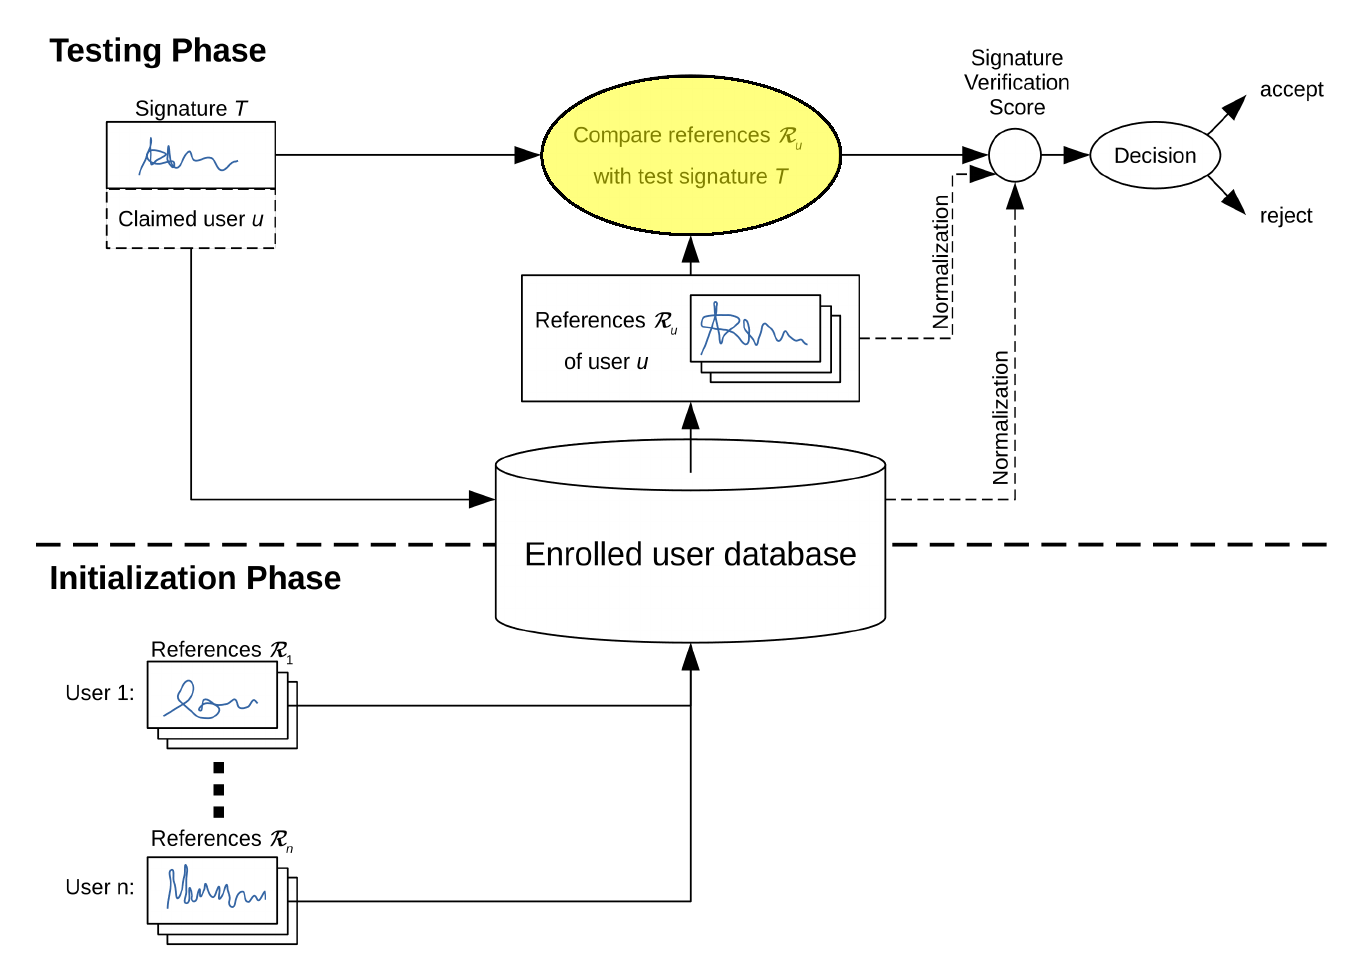
\includegraphics[width=0.7\textwidth]{12_verification_system}

\subsection{Neural network approach}

\begin{itemize}
		\item Extract 128-dimensional feature vector with neural network
		\item Compare those with euclidean distance, use that as dissimilarity
				score
		\item Vector space embedding groups similar signatures
		\item Triplet loss function: Loss based on anchor and positive from
				same user, and negative from another. Random triplets from
				training data. Training minimizes anchor-positive distance
				while maximizing anchor-negative distance.
		\item CNN used as able to utilize spatial information. Two pre-trained
				networks evaluated.
\end{itemize}

\subsubsection{Conlcusion}

\begin{itemize}
		\item Dissimilarity using CNN
		\item Embedding using triplet loss function
		\item Pretraining techniques reduces training cost
\end{itemize}

\subsection{Graph-based approach}

\subsubsection{Approximate signature as graph}

\begin{itemize}
		\item Skeletize via difference-of-gaussian, then binarization.
		\item Then pick points of interest on skeleton, e.g. endpoints, intersectinos, junctions, circles
		\item And evenly spaced points inbetween these
		\item Define graph using those
\end{itemize}

\subsubsection{Graph edit distance}

\begin{itemize}
		\item Minimal cost of transforming one graph into another using a set
				of basic edit operations: Substitution, deleting, insertion of
				nodes and edges.
		\item Each operation has a cost, which is minimized. In this case:
				\begin{itemize}
						\item Node substitution uses euclidean distance between the two
						\item Node insertion / deletion constant cost
						\item Edge substitution no cost
						\item Edge insertion / deletion constant cost
				\end{itemize}
		\item Algorithms solving GED have exponential complexity in number of
				nodes. Even basic signatures with low resolution quickly have
				many nodes!
		\item Two approxmations: Bipartite approximation (BP) with $O(n^3)$,
				Hausdorff Edit Distance (HED) with $O(n^2)$.
\end{itemize}

\paragraph{Bipartite approximation}

\begin{itemize}
		\item Two disjoint sets: Source graph and destination graph
		\item Find bijective mapping between a subset of each
		\item Each node on one side can be assigned to one node on other side,
				or be deleted
		\item Then pick cheapest option
\end{itemize}

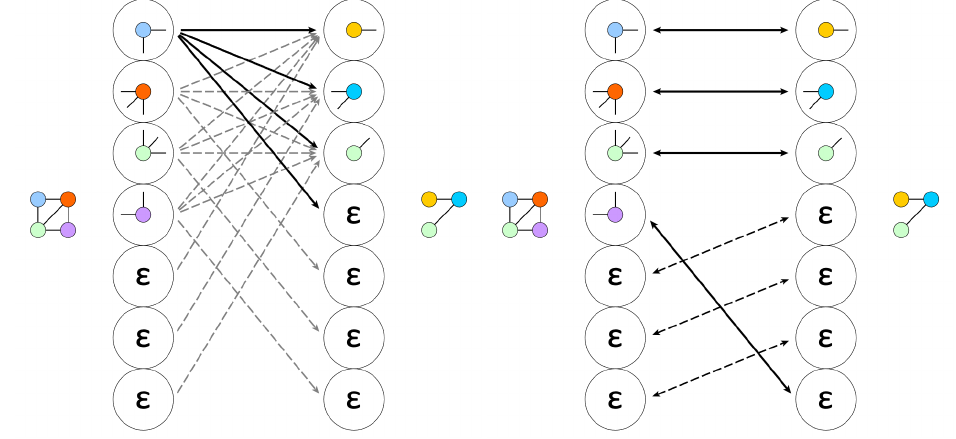
\includegraphics[width=0.6\textwidth]{12_bp}

\paragraph{Hausdorff Edit Distance}

\begin{itemize}
		\item Two sets as above
		\item Allow multiple assignments to same node
\end{itemize}

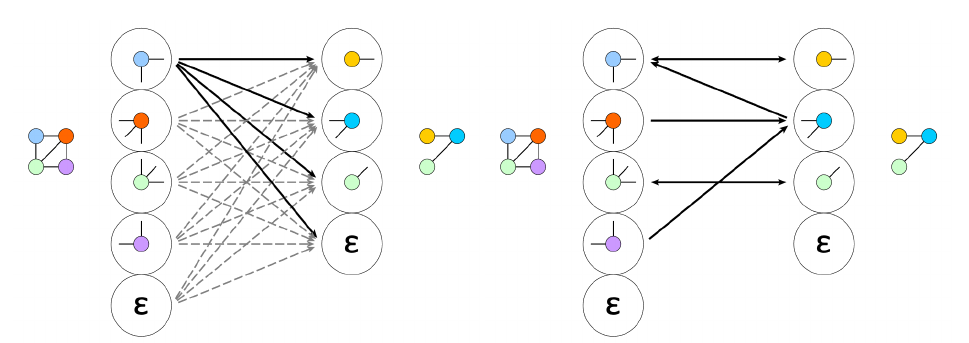
\includegraphics[width=0.6\textwidth]{12_hed}

\subsubsection{GED-based signature dissimilarity}

\[
		d_{GED}(R, T) = \frac{GED(g_R, g_T)}{GED_{max}(g_R, g_T)}
\]

$GED(R, T)$ (approximate) GED between $R, T$. $GED_{max}(R, T)$ is maximum-cost
GED, i.e. deleting all nodes/edges of $R$ and inserting all of $T$, used as
normalization technique. `Naive' edit path which is guaranteed to work.

Results showed that error much lower with normalization!

\paragraph{Results}

\begin{itemize}
		\item HED significantly faster than BP (let alone proper GED) while achieving similar EER
		\item Performance decreases if distance between points on graph gets
				too low (i.e. once approximation too exact, probably as it
				generalizes badly)
\end{itemize}

\subsection{Inkball model approach}

\begin{itemize}
		\item Inkball model is rooted tree
		\item Nodes are points on skeleton, edges to nearest nodes. Label
				specifies position relative to parent node.
		\item Minimize energy cost of tree
		\item Distance again uses normalization term
\end{itemize}

\subsection{Normalization}

\begin{itemize}
		\item User normalization normalizes within data of one user, improves
				performance
		\item Signature verification score normalization to allow combining
				GED, Inkball and CNN dissimilarities
\end{itemize}
